\documentclass[a4paper,12pt]{article}

\usepackage[utf8]{inputenc} 
\usepackage{amsmath}
\usepackage[a4paper, margin=0.8in, top=0.1in]{geometry} % Adjust the margin here
\usepackage{multirow}
\usepackage{nopageno}
\usepackage{graphicx} % Add this line to include graphics
\usepackage{wrapfig} % For wrapping figures
\usepackage{tikz}

\setlength{\parindent}{0pt} % Set global no indent
    
\title{{\large Department of Physics, FNSPE, CTU in Prague} \\
                  02YMECH - Mechanics \\ 
          {\Large \textbf{Make-up exam}}\vspace{-1cm}}
\date{14.1.2026 / 10:00 - 11:30}
\author{}

\begin{document}

\maketitle

\textbf{Q1:} Consider a system of two point particles, each having identical masses $m$, moving on a $xy$ plane with velocities, $\vec v_{1}~=~(0,at)$ and $\vec v_{2}~=~(at/2,0)$ where $a$, is a positive constant, and $t$ is time. The particles are initially in positions, $\vec r_{1}(0)~=~(1,0)$ and $\vec r_{2}(0)~=~(0,2)$.

\vspace*{0.1cm}
~(a) Find the total force and total torque about the origin. --- \textit{0.4 points}

~(b) Are total linear momentum and total angular momentum conserved? --- \textit{0.2 points}

~(c) Find the total kinetic energy in the LAB and center of mass frames. --- \textit{0.4 points}

\vspace*{0.25cm}
\textbf{Q2:} The equation of motion of a damped oscillator is given as $x(t)=e^{-\beta t}x_0\cos{\left(\omega_1 t\right)}$. How many oscillations $N$ does it approximately take for the amplitude of the oscillation to reduce to $1/2$? Express your result in terms of the quality factor $Q$, $\ln 2$ and $\pi$. Assume that the oscillator is weakly damped, i.e., $\omega_1 \approx \omega_0$.
(Givens: $Q = \omega_0/2\beta$, $T_0=2\pi/\omega_0$) --- \textit{1 point}

\vspace*{0.25cm}
\textbf{Q3:} A particle of mass $\mu$ moves under a central force $f(r)$ with angular momentum $l$. Its orbit is given by $r(\theta) = \frac{1}{a \theta^2}$ where $a > 0$. The orbit of a particle under a central force satisfies
\[
\frac{d^2}{d\theta^2}\left(\frac{1}{r}\right) + \frac{1}{r} = -\frac{\mu}{l^2} r^2 f(r).
\]

\vspace*{0.1cm}
~(a) Find the central force $f(r)$ in terms of $\mu$, $l$, and $r$. --- \textit{0.6 point}

~(b) Find the potential $U(r)$ associated with this force. --- \textit{0.4 point}

\vspace*{0.25cm}
\textbf{Q4:} A wagon of mass $m$ moves without friction along a straight, rigid rail fixed to a horizontal platform rotating with constant angular velocity $\Omega$.  
The rail is oriented radially outward from the axis of rotation and rotates together with the platform. Initially, the wagon is held at a distance $r_0$ from the axis of rotation and is at rest relative to the rail. It is then released and allowed to move freely along the rail.

\begin{wrapfigure}{r}{0.34\textwidth} % 'r' for right, width of figure box
    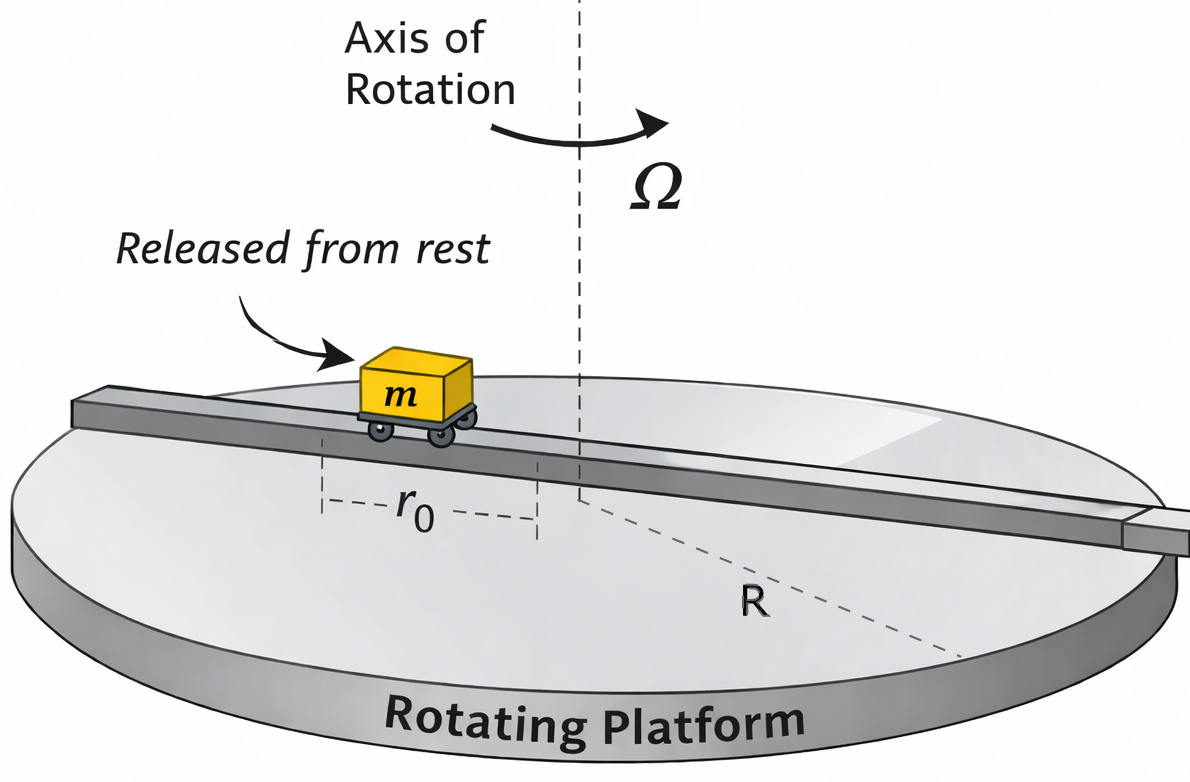
\includegraphics[width=\linewidth]{rot-rail.png} % use full width of wrapbox
\end{wrapfigure}

\vspace*{0.2cm}
~(a) In the reference frame rotating with the platform, write down the equation of motion for the wagon, including all inertial forces. --- \textit{0.5 point}

~(b) Solve the equation of motion to obtain $r(t)$. --- \textit{0.2 point}

~(c) Determine the time it takes for the wagon to reach the end of the rail located at radius $R>r_0$. --- \textit{0.2 point}

~(d) Explain physically why the wagon accelerates outward even though its initial velocity in the rotating frame is zero. --- \textit{0.1 point}

\underline{Givens}:
\begin{itemize}
    \item Coriolis force: $-2m(\vec{\Omega} \times \vec{v}')$
    \item Centrifugal force: $-m\vec{\Omega} \times (\vec{\Omega} \times \vec{r}')$
    \item $\cosh(x)=\frac{e^x + e^{-x}}{2}$
    \item Solution hypothesis for the equation $\ddot{x}\pm \omega^2 x=0$ is $x(t)=e^{\lambda t}$.
\end{itemize}


\end{document}

